% =============================================================================
% thesis-v5.tex
% 修士論文
%
% スポットインスタンス上の短時間ワークロードにおける
% 実行条件の選択による中断対策
%
% 構成:
%   第1章 序論（背景・既存研究・課題・目的）
%   第2章 関連研究
%   第3章 予備実験：SPS と継続性の関連  <- 実験中、結果は空欄
%   第4章 観測実験：中断特性の実測       <- DPS の内容
%   第5章 モデルの作成                   <- 定期分割の否定 + 実行条件選択
%   第6章 実証実験の設計
%   第7章 結論
%
% コンパイル: lualatex thesis-v5.tex (2回)
% =============================================================================
\documentclass[11pt,a4paper]{ltjsreport}

\usepackage{luatexja}
\usepackage{amsmath,amssymb}
\usepackage{graphicx}
\usepackage{booktabs}
\usepackage{tabularx}
\usepackage{array}
\usepackage{geometry}
\usepackage{caption}
\usepackage{url}
\usepackage[hidelinks]{hyperref}

\geometry{top=30mm,bottom=30mm,left=28mm,right=28mm}
\captionsetup[figure]{labelsep=quad,font=small}
\captionsetup[table]{labelsep=quad,font=small}

\newcommand{\Fcomp}{F_{\mathrm{comp}}}
\newcommand{\Rlaunch}{R_{\mathrm{launch}}}
\newcommand{\Rint}{R_{\mathrm{int}}}
\newcommand{\Nreq}{N_{\mathrm{req}}}
\newcommand{\Nsucc}{N_{\mathrm{succ}}}
\newcommand{\Nint}{N_{\mathrm{int}}}
\newcommand{\E}{\mathbb{E}}
\newcommand{\Waste}{\mathrm{Waste}}

% 未確定箇所を示すマーカー（提出前に削除する）
\newcommand{\TBD}[1]{\textbf{［#1］}}

\title{\vspace{-10mm}
スポットインスタンスにおける実測に基づく\\
実行条件選択モデルの構築}
\author{那須 渚}
\date{2026年度 修士論文\\[2mm] 同志社大学大学院 理工学研究科}

\begin{document}
\maketitle

% =============================================================================
\chapter*{概要}
\addcontentsline{toc}{chapter}{概要}

スポットインスタンスは，クラウドの余剰計算資源を
低価格で利用できる仕組みである．
しかし計算資源の空きが少なくなると，
\textbf{利用中のインスタンスが強制的に中断される}ことがある．
中断されると，それまでの処理を再実行する必要があり，
その分だけ実行時間と利用コストが増加する．
CI/CD のビルドやテストのような短時間ワークロードでは，
どの条件で実行すれば処理を完了できるかの判断が重要となる．

既存研究では，Spot Placement Score（SPS）を用いて
どこでスポットインスタンスを起動するかを選択する手法が
検討されてきた．
しかしこの指標が表すのは\textbf{起動のしやすさ}であり，
起動した後，\textbf{処理が終わるまで動き続けられるか}は
分からない．
本論文は予備実験によりこの点を確認したうえで，
プロバイダ固有の指標に依存せず
\textbf{実測値のみに基づいて実行条件を選択するモデル}を構築する．

まず，短時間ワークロードにおける信頼性指標として
\textbf{期限条件付き完了可能性} $\Fcomp(d)$，
すなわち起動に成功したインスタンスが
ワークロード期限 $d$ まで中断されずに利用可能であり続ける割合を定義し，
起動成功と起動後の中断挙動を分離して記録する
測定フレームワークを実装した．
AWS の 4 リージョン・3 インスタンスタイプを対象として
1 週間の観測実験（$\Nreq = 2{,}016$）を行った結果，
$\Fcomp(60)$ は実行条件によって $0.69$--$1.00$ の範囲で変動した．
また中断ハザード率は経過時間によらずほぼ一定であり，
\textbf{中断されやすさが稼働時間の長さではなく
実行条件によって決まる}ことを示した．

次に，この観測に基づき実行条件選択モデルを構築した．
中断による再実行で失われる時間を\textbf{損失時間}と定義し，
これを「やり直す回数」と「1 回あたりの中断時間」の積として定式化した．
両者はいずれも観測データから直接算出でき，
モデルの入力はすべて実測値である．
構築したモデルは，許容遅延の範囲で損失時間が最小となる
実行条件を選択する手続きを与える．

観測データを用いたシミュレーションによる評価の結果，
実行時刻を選択する戦略は，条件を選ばない場合に対して
損失時間を\textbf{$46\%$ 削減}し（許容遅延 6 時間のとき），
完了確率を $0.841$ から $0.883$ へ改善した．
また観測期間を分割し，一方の期間で条件を選択して
他方の期間で評価する検証を行い，
評価期間においても $30\%$ の削減を確認した．
これにより，効果が観測期間内の偶然によるものでないことを示した．

一方，リージョンおよびインスタンスタイプまで選択範囲を広げた場合には
より大きな削減が示唆されたが，
これは中断が一件も観測されなかった条件を選ぶことによるものであり，
標本数の制約から確定的な結論は得られない．
なお中断時の損失を抑える手法として定期分割も検討したが，
チェックポイントコストが大きい場合に成立せず，
またワークロードの改変を要するため採用しない．

ただし以上はいずれも観測データに基づくシミュレーション結果であり，
実環境での検証は行っていない．
この限界を明示したうえで，
構築したモデルを実環境で検証する実証実験の方法を示した．

% =============================================================================
\tableofcontents
\listoffigures
\listoftables

% =============================================================================
\chapter{序論}

\section{背景}
\label{sec:background}

近年，クラウドコンピューティングは企業，研究機関，個人開発者によって
広く利用されている．
クラウド利用の規模が拡大し，高性能な計算資源への需要が増加するにつれて，
その利用コストは多くの利用者にとって重要な課題となっている．

コストを削減する手法の一つに，スポットインスタンスの利用がある．
スポットインスタンスは，クラウドプロバイダが余剰計算資源を
オンデマンドインスタンスより低価格で提供する料金モデルである~\cite{AWSSpot}．
オンデマンドインスタンスと比較して，
数十パーセントから最大約 90\% の割引価格で利用できる~\cite{Lin2022Survey}．

この価格優位性から，スポットインスタンスは
機械学習やバッチ処理のような大規模計算ワークロードだけでなく，
CI/CD における自動ビルドやテストのように
一時的に計算資源を必要とするワークロードにも
利用されている~\cite{Ramesh2025}．

\subsection{スポットインスタンス利用の難しさ}

しかしスポットインスタンスは余剰容量に基づいて提供されるため，
\textbf{利用者の都合とは無関係に，
稼働中のインスタンスが中断されうる}．
クラウド需要が増加した場合や利用可能容量が減少した場合，
プロバイダは稼働中のインスタンスを回収する．
この中断を interruption event と呼ぶ．

中断がもたらす困難は，単に処理が停止することにとどまらない．

\paragraph{再実行による損失．}
ワークロードの実行中に中断が発生すると，
実行中の処理が完了前に停止する．
チェックポイントを取得していない場合，
それまでの処理内容は失われ，
ワークロード全体の再実行が必要となる．
その結果，実行時間と利用コストの双方が増加する．

\paragraph{予測の困難さ．}
中断がいつ発生するかを利用者が事前に知ることはできない．
プロバイダは中断の約 2 分前に警告を通知するが，
この猶予は保証されたものではなく，
また 2 分で完了できる対処は限られる．

\paragraph{条件による変動．}
中断のされやすさは，リージョン，インスタンスタイプ，
時間帯などの条件によって異なると考えられる．
しかし利用者がこの変動を把握する手段は限られている．

以上より，スポットインスタンスは価格面で有利である一方，
\textbf{どの条件で実行すれば安定して処理を完了できるか}を
判断することが難しい．
この判断の難しさが，
スポットインスタンス利用における中心的な課題である．

\section{既存研究}
\label{sec:existing}

この課題に対し，既存研究では
プロバイダが提供する指標を用いて実行先を選択する手法が検討されてきた．

その代表が Spot Placement Score（SPS）である~\cite{AWSSPS}．
SPS は AWS が提供する $1$ から $10$ の指標であり，
指定したインスタンスタイプ・リージョン・必要容量の条件下で
\textbf{スポットリクエストが成立する可能性}を推定するために用いられる．
スコアが高いほど，要求した容量を確保できる見込みが高い．

Katayama ら~\cite{Katayama2022} は，
マイグレーション先の選択に SPS を用いる手法を提案した．
中断が発生した際，SPS がより高いリージョンまたは
アベイラビリティゾーンへ移動することで，
再起動の成功率を高められることを示している．

また Kim ら~\cite{Kim2024SpotInterruption} は，
SPS が時間帯や曜日に応じて周期的に変動することを報告し，
スポットインスタンスの survival time との間に
一定の関係があることを示している．

これらの研究は，SPS が
\textbf{スポットインスタンスを起動できるかどうか}を判断するうえで
有用であることを示している．

\section{課題}
\label{sec:problem}

しかし，短時間ワークロードの利用者にとっての関心は，
起動できるかどうかだけではない．

\begin{quote}
\textbf{SPS は起動のしやすさを示す指標であり，
起動した後，処理が終わるまで動き続けられるか
--- 本論文ではこれを\emph{起動の継続性}と呼ぶ --- を
示す指標ではない．}
\end{quote}

スポットリクエストが成立することと，
ワークロードが完了することは異なる問題である．
たとえ起動に成功したとしても，
ワークロードの完了前に中断されれば，
短時間ワークロードは失敗する．

この違いは，CI/CD パイプラインや
短時間バッチ処理のようなワークロードにおいて特に重要である．
これらは比較的短い実行時間を持つが，
完了前に中断された場合はジョブ全体の再実行が必要となり，
実行時間と運用コストの双方が増加する．

したがって利用者に必要なのは，
\textbf{要求される実行時間の期限までインスタンスが
利用可能な状態を維持できるか}に関する情報である．

本論文では，この課題に対して二段階で取り組む．

\begin{enumerate}
  \item \textbf{SPS の限界の確認}（第~\ref{chap:prelim} 章）：
        SPS と起動後の継続性との関連を予備実験により検証し，
        SPS が継続性の指標として十分でないことを確かめる．
  \item \textbf{実測に基づく指標の構築}（第~\ref{chap:measure} 章以降）：
        プロバイダ固有の指標に依存せず，
        直接観測された起動・中断記録のみから算出される
        信頼性指標を定義し，これに基づく実行条件の選択手法を構築する．
\end{enumerate}

\section{目的}
\label{sec:objective}

本論文の目的は次の通りである．

\begin{quote}
\textbf{実測値による観測に基づき，
中断によって失われる時間を最小化する実行条件を
決定する手法を確立する．}
\end{quote}

ここで「実測値による観測」を基礎とするのは，
第~\ref{sec:problem} 節で述べた課題に対応するためである．
プロバイダ固有の指標は，その算出根拠が公開されておらず，
また起動の継続性を直接には示さない．
これに対し，自ら観測した起動・中断記録は，
算出根拠が明確であり，
かつ関心のある量（期限までの継続性）を直接測定できる．

目的を達成するため，本論文では次の四つの段階を踏む．

\begin{enumerate}
  \item 予備実験により SPS の限界を確認する（第~\ref{chap:prelim} 章）
  \item 実測により中断特性を把握する（第~\ref{chap:measure} 章）
  \item 実測値に基づくモデルを構築する（第~\ref{chap:model} 章）
  \item モデルを検証する実証実験を設計する（第~\ref{chap:exp} 章）
\end{enumerate}

\section{本論文の貢献}

本論文の貢献は以下の通りである．

\begin{enumerate}
  \item SPS が起動の継続性を示す指標として十分でないことを，
        予備実験により確認した（第~\ref{chap:prelim} 章）．
  \item 短時間ワークロードにおける信頼性を，
        実測値のみから算出される
        \textbf{期限条件付き完了可能性} $\Fcomp(d)$ として定義し，
        起動成功と起動後の中断挙動を分離して記録する
        測定フレームワークを実装した（第~\ref{chap:measure} 章）．
  \item 4 リージョン・3 インスタンスタイプ・1 週間の実測により，
        $\Fcomp(d)$ が実行条件によって大きく変動すること，
        および\textbf{中断ハザード率が経過時間によらずほぼ一定}であることを
        示した（第~\ref{chap:measure} 章）．
  \item 実測値のみを入力とする\textbf{実行条件選択モデル}を構築し，
        実行時刻の選択により損失時間が $46\%$ 削減されること，
        および期間を分割した検証でも $30\%$ の削減が
        確認されることを示した（第~\ref{chap:model} 章）．
  \item 構築したモデルを実環境で検証する
        実証実験の方法を示した（第~\ref{chap:exp} 章）．
\end{enumerate}

\section{本論文の構成}

第~\ref{chap:related} 章では関連研究を整理する．
第~\ref{chap:prelim} 章では SPS に関する予備実験を述べる．
第~\ref{chap:measure} 章では観測実験の内容と結果を示す．
第~\ref{chap:model} 章では実行条件選択モデルを構築する．
第~\ref{chap:exp} 章では実証実験の方法を示す．
第~\ref{chap:conclusion} 章で本論文をまとめる．

% =============================================================================
\chapter{関連研究}
\label{chap:related}

\section{スポットインスタンスの可用性向上手法}

Lin ら~\cite{Lin2022Survey} は
スポットインスタンスの可用性を向上させる手法を調査し，
チェックポイント，マイグレーション，レプリケーション，
スケジューリングといったアプローチを整理している．
これらの研究は，スポットインスタンスを実用的に利用するうえで
中断リスクが中心的課題であることを示している．

本研究が扱う実行条件の選択は，
この分類におけるスケジューリングに相当する．
一方，第~\ref{chap:model} 章で検討する定期分割は
チェックポイントに相当する．

\section{プロバイダ固有の指標に基づく選択}

SPS は AWS が提供するプロバイダ固有の指標であり，
スポットリクエストが成立する可能性を推定するために
用いられる~\cite{AWSSPS}．

Katayama ら~\cite{Katayama2022} は
マイグレーション先の選択に SPS を用い，
起動時点の可用性を向上させられることを示した．
また Garg ら~\cite{Garg2025} は
価格変動を考慮した入札戦略を検討している．

これらの手法は，起動時点の可用性やコストの観点からは有効である．
しかし\S\ref{sec:problem} で述べたとおり，
起動に成功したインスタンスが
ワークロードを完了するのに十分な時間
利用可能な状態を維持できるかどうかは，
これらの指標からは直接判断できない．

\section{中断挙動の観測と分析}

Kim ら~\cite{Kim2024SpotInterruption} は，
SPS が時間帯や曜日に応じて周期的に変動し，
survival time と一定の関係を持つことを示している．
Lee ら~\cite{Lee2022SpotLake} は，SPS，スポット価格，中断率などを
継続的に収集・保存するアーカイブサービス SpotLake を提案し，
GPU インスタンスや大規模インスタンスタイプで
可用性が低くなる傾向があることを報告している．

これらの研究は中断挙動の統計的性質を明らかにしている．
ただし時間的変動は主として
\textbf{観測・記述の対象}として扱われており，
観測された変動を
\textbf{実行条件を選択するための入力}として用いる枠組みは
十分に検討されていない．

\section{本研究の位置づけ}

既存研究に対する本研究の位置づけを表~\ref{tab:related} に示す．

\begin{table}[htbp]
\centering
\caption{関連研究と本研究の位置づけ}
\label{tab:related}
\small
\begin{tabularx}{\textwidth}{@{}lXX@{}}
\toprule
 & \textbf{用いる指標} & \textbf{指標の用途} \\
\midrule
SPS~\cite{AWSSPS}，
Katayama ら~\cite{Katayama2022}
  & プロバイダ固有（起動可能性）
  & 起動先の選択 \\
\addlinespace
Kim ら~\cite{Kim2024SpotInterruption}，
Lee ら~\cite{Lee2022SpotLake}
  & 観測データ（中断率，survival time）
  & 現象の記述・分析 \\
\addlinespace
\textbf{本研究}
  & \textbf{観測データ（期限条件付き完了可能性）}
  & \textbf{実行条件の決定} \\
\bottomrule
\end{tabularx}
\end{table}

% =============================================================================
\chapter{予備実験：SPS と起動の継続性}
\label{chap:prelim}

\section{本章のねらい}

\S\ref{sec:problem} で述べたとおり，
本研究は「SPS は起動のしやすさを示す指標であり，
起動の継続性を示す指標ではない」という課題認識に立つ．

本章ではこの認識を実測により確認する．
具体的には，スポットインスタンスの起動時に SPS を記録し，
その後の稼働状況との関連を分析する．

\paragraph{本章の位置づけ．}
本章の結果は，第~\ref{chap:measure} 章以降で
\textbf{実測値に基づく独自の指標を構築する理由}を与える．
もし SPS が継続性とも強く関連するのであれば，
新たな指標を定義する必要性は小さい．
逆に関連が弱いのであれば，
継続性を直接測定する指標が必要となる．

\section{実験方法}

\subsection{測定項目}

スポットインスタンスの起動リクエスト時に，
対象のインスタンスタイプ・リージョン・
アベイラビリティゾーンに対する SPS を取得し，
起動結果および稼働状況とあわせて記録する．

\begin{table}[htbp]
\centering
\caption{予備実験の測定項目}
\label{tab:prelim_items}
\small
\begin{tabularx}{\textwidth}{@{}lX@{}}
\toprule
項目 & 内容 \\
\midrule
SPS & 起動リクエスト時に取得したスコア（$1$--$10$） \\
起動成否 & リクエストが成立したか \\
稼働時間 & 起動から中断または正常終了までの時間 \\
中断の有無 & 観測期間内に中断されたか \\
\bottomrule
\end{tabularx}
\end{table}

SPS はアベイラビリティゾーン単位で取得する．
AWS の API はゾーン ID（\texttt{apne1-az3} 等）で応答するため，
ゾーン名との対応を変換して記録する．

\subsection{分析の方針}

SPS と以下の二つの量との関連をそれぞれ分析する．

\begin{enumerate}
  \item \textbf{起動成功率との関連}：
        SPS が本来示すとされる量である．
        正の関連が認められることを確認する．
  \item \textbf{起動後の継続性との関連}：
        本研究の関心事である．
        起動に成功したインスタンスに限定し，
        SPS と中断の有無および稼働時間との関連を分析する．
\end{enumerate}

分析 1 で関連が認められ，分析 2 で認められない場合，
\textbf{SPS は起動可能性の指標ではあるが
継続性の指標ではない}という本研究の課題認識が支持される．

\section{実験結果}
\label{sec:prelim_result}

\TBD{本節は実験実施中である。結果が得られ次第記述する。}

\subsection{SPS と起動成功率の関連}

\TBD{SPS の値ごとの起動成功率を示す表・図を挿入}

\TBD{相関の有無と、その解釈を記述}

\subsection{SPS と起動後の継続性の関連}

\TBD{SPS の値ごとの中断率・平均稼働時間を示す表・図を挿入}

\TBD{相関の有無と、その解釈を記述}

\section{考察}

\TBD{結果を踏まえた考察を記述}

\TBD{想定される記述：SPS は起動成功率とは関連するが、
起動後の継続性とは明確な関連を示さない。
したがって、短時間ワークロードの完了可能性を判断するには
SPS では不十分であり、継続性を直接測定する指標が必要である。}

\section{本章のまとめ}

\TBD{結果を踏まえて記述}

本章の結果は，次章以降で
\textbf{実測値に基づく独自の信頼性指標}を構築する動機となる．

% =============================================================================
\chapter{観測実験：中断特性の実測}
\label{chap:measure}

\section{本章のねらい}

第~\ref{chap:prelim} 章の結果を踏まえ，
本章ではプロバイダ固有の指標に依存せず，
\textbf{直接観測された記録のみから算出される}
信頼性指標を定義し，実測を行う．

得られたデータは，第~\ref{chap:model} 章で構築するモデルの
入力となる．具体的には，実行条件ごとの

\begin{itemize}
  \item 期限 $d$ まで中断されずに完了する確率
  \item 中断された場合に失われる時間の期待値
  \item インスタンスの起動オーバーヘッド
\end{itemize}

を取得する．

\section{期限条件付き完了可能性}

\subsection{指標の定義}

本研究では実際のアプリケーションレベルのワークロードは実行しない．
代わりに，指定期限まで中断されずに利用可能であることを
\textbf{ワークロード完了可能性の proxy} として用いる．
すなわち，起動に成功したインスタンスが期限 $d$ より前に
中断されなかった場合，観測条件下において
その実行時間要件を持つ短時間ワークロードは完了可能とみなす．

$\Nreq$ をスポットインスタンスの起動リクエスト数，
$\Nsucc$ を起動に成功したインスタンス数，
$\Nint(d)$ を期限 $d$ より前に中断された
起動成功インスタンス数とする．

\textbf{起動成功率}を次のように定義する．

\begin{equation}
\Rlaunch = \frac{\Nsucc}{\Nreq}
\label{eq:rlaunch}
\end{equation}

\textbf{期限前中断率}を次のように定義する．

\begin{equation}
\Rint(d) = \frac{\Nint(d)}{\Nsucc}
\label{eq:rint}
\end{equation}

さらに\textbf{期限条件付き完了可能性}を次のように定義する．

\begin{equation}
\boxed{\;\Fcomp(d) = 1 - \Rint(d)\;}
\label{eq:fcomp}
\end{equation}

この指標は，起動に成功したインスタンスのうち
期限 $d$ まで利用可能な状態を維持した割合を表す．

\subsection{SPS との関係}

式~\eqref{eq:rlaunch} と式~\eqref{eq:rint} を
分離して定義することにより，
\textbf{起動時点の可用性}と\textbf{起動後の継続性}を
区別して分析できる．

この区別は，第~\ref{chap:prelim} 章で扱った課題に対応する．
SPS が対象とするのは前者であり，
$\Fcomp(d)$ が対象とするのは後者である．
両者は排他的ではなく，
スポットインスタンスの信頼性の異なる側面を捉える
相補的な指標である．

\section{測定フレームワーク}

図~\ref{fig:framework} に測定フレームワークを示す．

\begin{figure}[htbp]
\centering
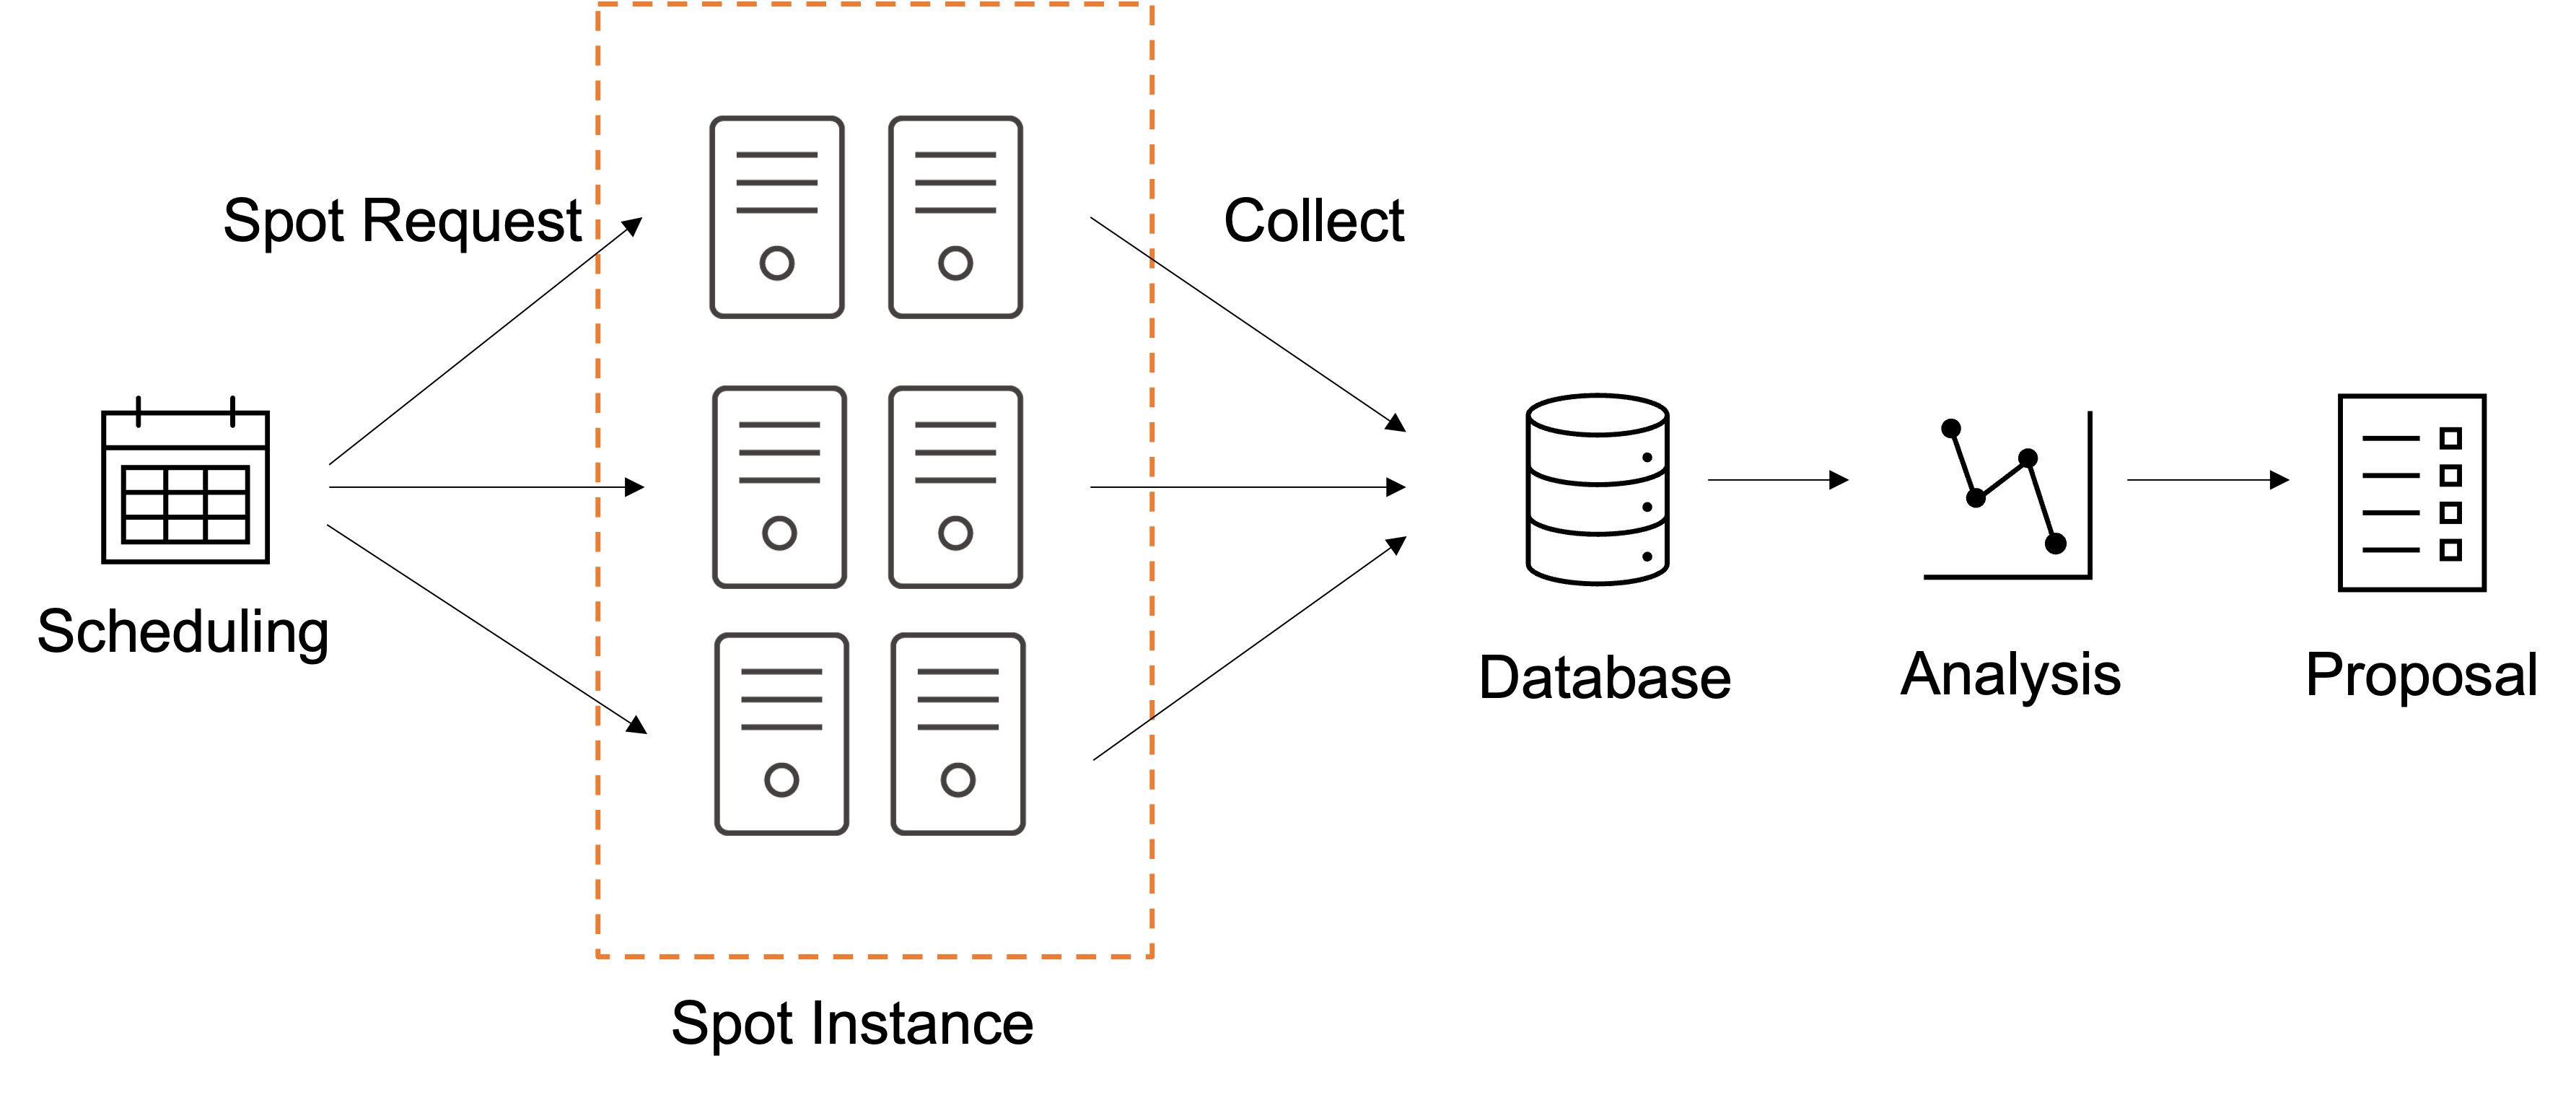
\includegraphics[width=\textwidth]{images/artect.png}
\caption{測定フレームワーク}
\label{fig:framework}
\end{figure}

スケジューラは対象とする各インスタンスタイプに対して
定期的に起動リクエストを送信する．
起動に成功した各インスタンスは 1 時間の固定観測期間にわたって監視される．
この期間中，システムはリクエストが成立したか，
インスタンスがどの程度の時間利用可能であったか，
予定終了時刻より前に中断が発生したかを記録する．
観測期間内に中断が発生しなかった場合，
インスタンスはシステムによって終了される．

スポット中断と通常のシステム終了を区別するため，
測定システムによって終了されることなく
予定された 1 時間の観測終了前に利用不能となったインスタンスを
中断候補として扱う．

\section{実験設定}

\paragraph{インスタンスタイプ．}
異なるリソース特性を持つインスタンスタイプ間で中断傾向を比較するため，
3 種類を代表例として選定した~\cite{Pham2018,AWSInstanceTypes}．
仕様を表~\ref{tab:specs} に示す．

\begin{table}[htbp]
\centering
\caption{評価対象インスタンスタイプの仕様。観測スポット価格は観測期間中
（2026年5月19日--25日）に 4 リージョンで記録された平均時間単価（USD/h）である。}
\label{tab:specs}
\small
\begin{tabularx}{\textwidth}{@{}l>{\raggedright\arraybackslash}X>{\raggedright\arraybackslash}X>{\raggedright\arraybackslash}X@{}}
\toprule
 & \textbf{c6a.large} & \textbf{g4dn.xlarge} & \textbf{t3.micro} \\
\midrule
分類 & 計算最適化 & GPU 搭載 & バースト可能汎用 \\
プロセッサ & AMD EPYC (3rd gen) & Intel Xeon (Cascade Lake) & Intel Xeon (burstable) \\
vCPU & 2 & 4 & 2 (burstable) \\
メモリ & 4 GiB & 16 GiB & 1 GiB \\
GPU & --- & 1$\times$ NVIDIA T4 (16 GiB) & --- \\
ローカルストレージ & EBS のみ & 125 GB NVMe SSD & EBS のみ \\
観測スポット価格 & 0.038 & 0.277 & 0.005 \\
\bottomrule
\end{tabularx}
\end{table}

\paragraph{リージョンと時間帯．}
対象リージョンは N.~Virginia (us-east-1)，Tokyo (ap-northeast-1)，
Ireland (eu-west-1)，Singapore (ap-southeast-1) の 4 つである．
各リージョンにおいて，各インスタンスタイプにつき 1 時間に 1 台を起動する．

タイムスタンプを各リージョンのローカル時刻に正規化したうえで，
ローカル 1 日を 6 時間ずつの 4 区間に分割して記録する
（表~\ref{tab:periods}）．

\begin{table}[htbp]
\centering
\caption{ローカル時間帯の区分}
\label{tab:periods}
\small
\begin{tabular}{@{}ll@{}}
\toprule
区分 & ローカル時刻 \\
\midrule
Night     & 00:00--05:59 \\
Morning   & 06:00--11:59 \\
Afternoon & 12:00--17:59 \\
Evening   & 18:00--23:59 \\
\bottomrule
\end{tabular}
\end{table}

\paragraph{観測期間と価格設定．}
実験は 2026 年 5 月 19 日から 5 月 25 日まで実施した．
スポットリクエストでは最大スポット価格を指定していない．

\section{実験結果}

\subsection{全体の傾向}

観測期間中，4 リージョン・3 インスタンスタイプにわたり
合計 $\Nreq = 2{,}016$ 件の起動リクエストを送信した．
このうち $\Nsucc = 1{,}950$ 件が正常に起動し，
全体の起動成功率は $\Rlaunch = 96.7\%$ であった．
起動に成功したインスタンスのうち 117 件（$6.0\%$）が
1 時間の観測期間終了前に中断された．

期限 $d$ ごとの $\Fcomp(d)$ を表~\ref{tab:fcomp_overall} に示す．

\begin{table}[htbp]
\centering
\caption{期限 $d$ ごとの $\Fcomp(d)$（全データをプール，$\Nsucc = 1{,}950$）}
\label{tab:fcomp_overall}
\small
\begin{tabular}{@{}lrrrr@{}}
\toprule
期限 $d$ & 5 分 & 10 分 & 30 分 & 60 分 \\
\midrule
$\Fcomp(d)$ & 0.9938 & 0.9882 & 0.9692 & 0.9451 \\
\bottomrule
\end{tabular}
\end{table}

\subsection{実行条件による変動}
\label{sec:variation}

図~\ref{fig:heatmap60} に，時間帯，リージョン，
インスタンスタイプごとに集計した $\Fcomp(60)$ を示す．

\begin{figure}[htbp]
\centering
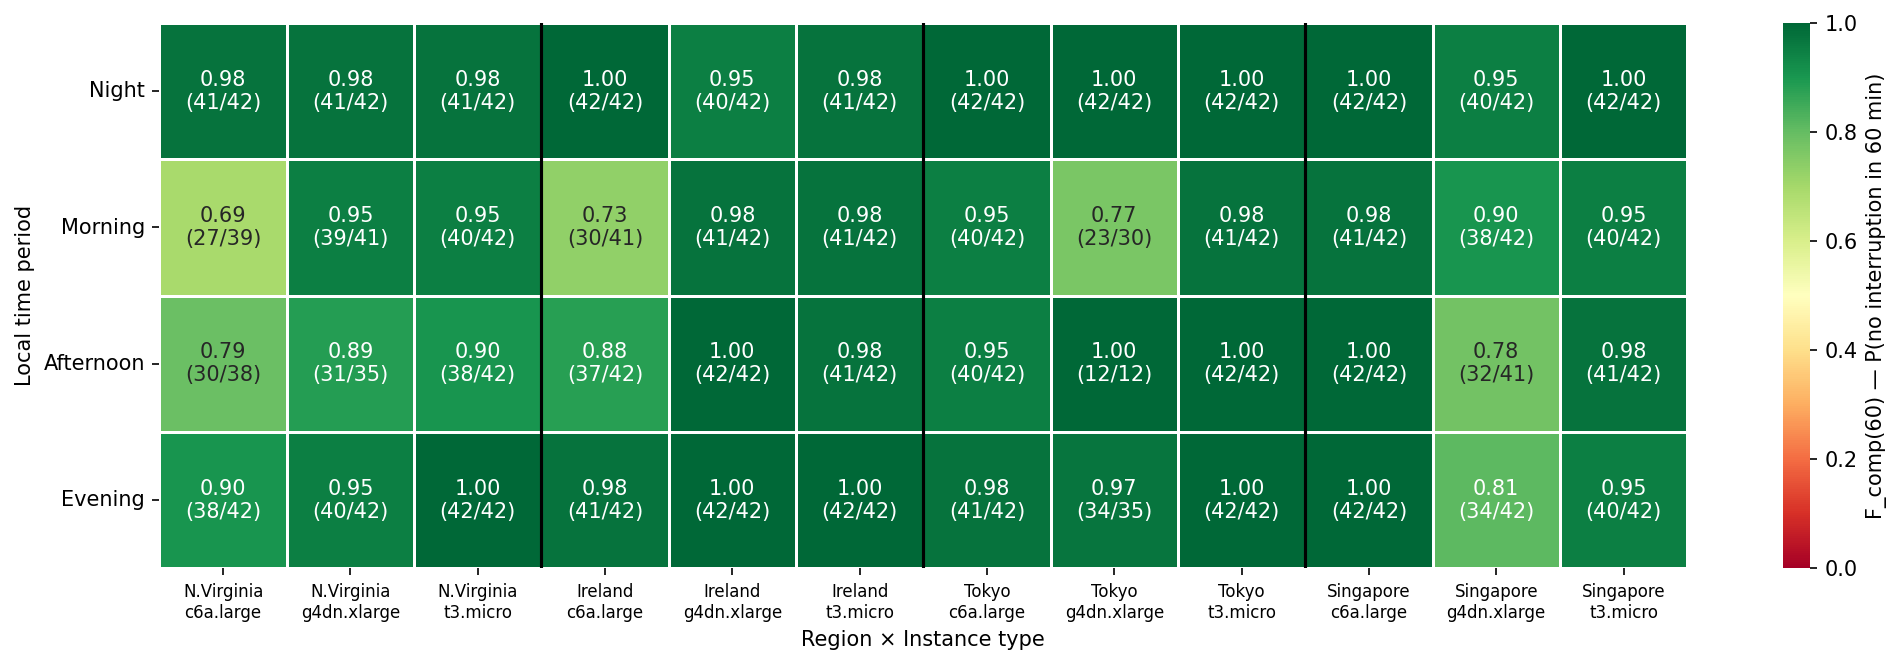
\includegraphics[width=\textwidth]{images/figure1_fcomp60_heatmap.png}
\caption{時間帯，リージョン，インスタンスタイプ別の $\Fcomp(60)$。
注釈は値とサンプル数（$n_{\mathrm{comp}}/n_{\mathrm{succ}}$）を示す。}
\label{fig:heatmap60}
\end{figure}

t3.micro はすべての条件において $\Fcomp(60) \geq 0.95$ を達成しており，
軽量インスタンスは中断に対して比較的頑健であることを示している．
一方 c6a.large および g4dn.xlarge では条件による変動が大きく，
値はおおよそ 0.65 から 1.00 の範囲で変化した．

最大の変動は N.~Virginia の c6a.large において観測された．
時間帯別の値を表~\ref{tab:period_var} に示す．

\begin{table}[htbp]
\centering
\caption{N.~Virginia，c6a.large における時間帯別の $\Fcomp(60)$}
\label{tab:period_var}
\small
\begin{tabular}{@{}lrrr@{}}
\toprule
時間帯 & $\Fcomp(60)$ & 95\% 信頼区間 & $n$ \\
\midrule
Night     & 0.98 & 0.88--1.00 & 42 \\
Morning   & 0.69 & 0.54--0.81 & 39 \\
Afternoon & 0.79 & 0.64--0.89 & 38 \\
Evening   & 0.91 & 0.78--0.96 & 42 \\
\bottomrule
\end{tabular}
\end{table}

Night と Morning の差は約 0.29 であり，
両者の信頼区間は重ならない．
この差が標本変動に起因する可能性は低い．

観測された傾向は，ローカルなクラウド需要が
日内周期に従うという仮説と整合する．
最もリスクの高い時間帯がリージョンによって異なることも
この解釈を支持する．
N.~Virginia と Ireland では Morning が最もリスクが高く，
これは北米および欧州の業務開始時間帯と対応する．
Singapore では Afternoon が最もリスクが高く，
アジア地域の午後の利用ピークと整合する．

\subsection{中断ハザード率の挙動}
\label{sec:hazard}

中断が経過時間に対してどのように発生するかを分析した．
経過時間区間ごとに，その区間に入る直前まで生存していた
インスタンス数（リスク集合）で正規化したハザード率を
表~\ref{tab:hazard} および図~\ref{fig:hazard} に示す．

\begin{table}[htbp]
\centering
\caption{経過時間別の中断ハザード率（$\Nsucc = 1{,}950$，中断 117 件）}
\label{tab:hazard}
\small
\begin{tabular}{@{}lrrrr@{}}
\toprule
経過時間 & 中断件数 & リスク集合 & 区間あたり & 単位時間あたり \\
\midrule
0--5 分   & 12 & 1,950 & 0.62\% & 0.123 \%/分 \\
5--10 分  & 11 & 1,938 & 0.57\% & 0.114 \%/分 \\
10--20 分 & 25 & 1,927 & 1.30\% & 0.130 \%/分 \\
20--30 分 & 12 & 1,902 & 0.63\% & 0.063 \%/分 \\
30--40 分 & 14 & 1,890 & 0.74\% & 0.074 \%/分 \\
40--50 分 & 23 & 1,876 & 1.23\% & 0.123 \%/分 \\
50--60 分 & 10 & 1,853 & 0.54\% & 0.054 \%/分 \\
\bottomrule
\end{tabular}
\end{table}

\begin{figure}[htbp]
\centering
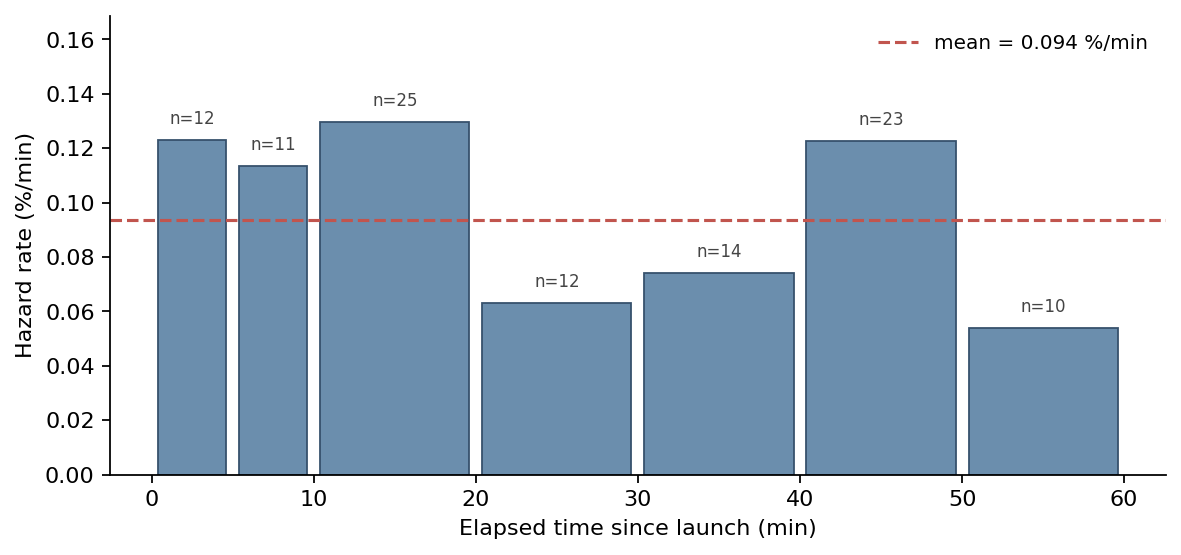
\includegraphics[width=0.85\textwidth]{images/figure3_hazard.png}
\caption{経過時間別の中断ハザード率。単調増加の傾向は見られず，
0.054--0.130 \%/分の範囲で変動する。}
\label{fig:hazard}
\end{figure}

ハザード率は 0.054--0.130 \%/分の範囲で変動するが，
\textbf{経過時間に対する単調増加の傾向は見られない}．
すなわち「長時間稼働したインスタンスほど中断されやすくなる」
という摩耗的な性質は観測されない．
中断は単位時間あたりほぼ一定の確率で発生する，
近似的にメモリレスな事象として振る舞う．

この性質は，第~\ref{chap:model} 章で検討する
二つのモデルの出発点となる．

\paragraph{この主張の限界．}
中断 117 件という標本数のもとでは，
ハザードの定数性を統計的に強く主張することはできない．
本論文では「単調増加の証拠が得られなかった」という
弱い主張にとどめる．

\subsection{起動オーバーヘッド}

インスタンスの起動リクエストから実行開始までに要した時間は，
平均 $4.52$ 秒（中央値 $4$ 秒，95 パーセンタイル $6$ 秒，
最大 $30$ 秒）であった．
この値は第~\ref{chap:model} 章のモデルにおいて用いる．

\section{本章の限界}
\label{sec:limit_measure}

\begin{itemize}
  \item 観測期間は 1 週間に限定されており，
        各条件のサンプル数は 30--42 である．
        結果は短期的変動を反映している可能性がある．
  \item 中断されない状態を完了可能性の proxy としており，
        実際のアプリケーションレベルのワークロードは実行していない．
  \item 各条件につき 1 時間に 1 台のみ起動しているため，
        同時起動の影響やキュー挙動は捉えられていない．
  \item 最大スポット価格を指定していないため，
        デフォルト価格設定下の挙動のみを反映している．
\end{itemize}

\section{本章のまとめ}

\begin{enumerate}
  \item 起動成功率 $96.7\%$，中断率 $6.0\%$ を観測した．
  \item $\Fcomp(60)$ は実行条件によって $0.69$--$1.00$ の範囲で変動する．
        最大の差は N.~Virginia の c6a.large における
        Night と Morning の間の $0.29$ であり，信頼区間は重ならない．
  \item 中断ハザード率は経過時間によらずほぼ一定である．
  \item 起動オーバーヘッドは平均 $4.52$ 秒である．
\end{enumerate}

% =============================================================================
\chapter{実行条件選択モデルの構築}
\label{chap:model}

\section{本章のねらい}

第~\ref{chap:measure} 章の観測から，
中断対策として二つの方向が考えられる．

\paragraph{方向 1：中断時の損失を減らす（定期分割）.}
\S\ref{sec:hazard} で示したハザード率の一定性は，
\textbf{実行単位を短くすれば中断に遭遇しにくくなる}
ことを含意する．
そこでジョブを分割し，チェックポイントで接続すれば，
中断時に失われる時間を抑えられる可能性がある．

\paragraph{方向 2：中断されにくい条件を選ぶ（実行条件選択）.}
\S\ref{sec:variation} で示した条件による変動は，
\textbf{適切な条件を選べば中断されにくくなる}
ことを含意する．

本章では，まず方向 1（定期分割）を検討し，
適用範囲が限定されるため採用しないことを示す（\S\ref{sec:split}）。
そのうえで方向 2（実行条件選択）のモデルを構築し，
評価する（\S\ref{sec:selection} 以降）。

\paragraph{共通の枠組み：損失時間．}
両モデルの比較のため，共通の評価量を定める．
中断されるとジョブは再実行されるため，
利用者が支払う総時間は本来必要な計算時間を上回る．
この超過分を\textbf{損失時間}と呼び，最小化対象とする．

損失時間は二つの要素の積として表される．

\begin{equation}
\text{損失時間} \;=\;
\underbrace{\text{やり直す回数}}_{\text{中断されにくさで決まる}}
\;\times\;
\underbrace{\text{1 回あたりの中断時間}}_{\text{中断までの経過時間で決まる}}
\label{eq:waste_concept}
\end{equation}

方向 1 は第二要素を，方向 2 は第一要素を削減する手法として
位置づけられる．

\section{検討から除外した手法：定期分割}
\label{sec:split}

本節では，もう一方の方向である定期分割を検討し，
これを採用しない理由を示す。

\subsection{定式化と最適分割数}

総計算量 $W$ のジョブを $k$ 個の断片に分割し，
チェックポイントで接続することを考える．
1 断片の長さは $T = W/k$ となり，総損失時間は

\begin{equation}
\Waste(k)
=
k \left( \frac{1}{p(T)} - 1 \right) \bar u(T)
\;+\;
k\,(s + c)
\label{eq:waste_split}
\end{equation}

で与えられる．
ここで $c$ はチェックポイントの保存および復元コストである．
第 1 項は $k$ の増加とともに減少し，第 2 項は $k$ に比例して増加するため，
$\Waste$ は $k$ に対して U 字型となり，
\textbf{最適分割数 $k^{*}$ が存在する}．

第~\ref{chap:measure} 章のデータを適用した結果を
表~\ref{tab:split_summary} に示す．

\begin{table}[htbp]
\centering
\caption{定期分割の総損失時間（$W = 60$ 分）。
太字は各行の最小値を示す。$c$ はチェックポイントコストである。}
\label{tab:split_summary}
\small
\begin{tabular}{@{}rrrrrrc@{}}
\toprule
$c$ (秒) & $k{=}1$ & $k{=}2$ & $k{=}4$ & $k{=}6$ & $k{=}12$ & $\mathbf{k^{*}}$ \\
\midrule
0   & 1.94 & 1.19 & 1.21 & \textbf{0.98} & 1.20 & \textbf{6} \\
5   & 2.02 & \textbf{1.36} & 1.54 & 1.48 & 2.20 & \textbf{2} \\
30  & 2.44 & \textbf{2.19} & 3.21 & 3.98 & 7.20 & \textbf{2} \\
60  & \textbf{2.94} & 3.19 & 5.21 & 6.98 & 13.20 & \textbf{1} \\
180 & \textbf{4.94} & 7.19 & 13.21 & 18.98 & 37.20 & \textbf{1} \\
\bottomrule
\end{tabular}
\end{table}

チェックポイントが無償（$c = 0$）であれば
$k^{*} = 6$ において $50\%$ の削減が得られる．
しかし $c$ の増加とともに $k^{*}$ は急速に低下し，
$c \geq 60$ 秒では $k^{*} = 1$ となって
\textbf{分割による利得が完全に失われる}．
さらに $c = 180$ 秒のもとで $k = 6$ とした場合，
損失時間は $18.98$ 分に達し，
分割しない場合（$1.94$ 分）の\textbf{約 $10$ 倍}となる．

\subsection{採用しない理由}
\label{sec:why_not_split}

以上を踏まえ，本研究では定期分割を採用しない．理由は二つある．

\paragraph{理由 1：適用範囲が限定される．}
定期分割が有効なのは $c < 60$ 秒の場合に限られる．
保存すべき状態が大きいワークロードではこの条件を満たさず，
むしろ損失時間を増大させる．
定期的なチェックポイント取得は
スポットインスタンス利用の定石として広く行われているが，
\textbf{条件によってはこの慣行が有害となる}．

\paragraph{理由 2：ワークロードの改変を要する．}
定期分割は，処理の途中で一貫した状態を保存し，
別のインスタンスで復元できることを前提とする．
この機構を実装できないワークロードには適用できない．

\paragraph{実行条件選択との対比．}
次節で扱う実行条件の選択は，
チェックポイントコストの影響を受けず，
ワークロードの改変も必要としない．
両手法の理想条件下での削減率は同程度であるが
（定期分割 $50\%$，実行条件選択 $46\%$），
条件を満たさない場合の挙動が異なる．
定期分割が最大 $10$ 倍の悪化をもたらすのに対し，
実行条件の選択は効果が得られないにとどまる．
本研究が後者を採用するのは，この非対称性による．

\section{実行条件選択のモデル}
\label{sec:selection}

\subsection{モデル化の方針}
\label{sec:model_policy}

モデルを構築するにあたり，三つの設計判断を行った．

\paragraph{判断 1：最小化対象は損失時間とする．}
最小化対象として利用料金（USD）も考えられるが，
本研究は損失時間（分）を採用する．

料金を目的関数とすると，
リージョン間の価格差が中断特性の差を覆い隠すためである．
表~\ref{tab:price_gap} に示すとおり，
c6a.large のリージョン間価格差は $34$--$41\%$ に達する．
一方，中断による課金時間の増加は数パーセントにとどまる．
したがって料金を最小化すれば，
中断特性によらず常に最安リージョンが選ばれ，
中断対策としての意味を失う．

\begin{table}[htbp]
\centering
\caption{c6a.large のリージョン別観測スポット価格}
\label{tab:price_gap}
\small
\begin{tabular}{@{}lrr@{}}
\toprule
リージョン & 価格 (USD/h) & N.~Virginia 比 \\
\midrule
N.~Virginia & 0.0295 & --- \\
Singapore   & 0.0394 & $+34\%$ \\
Ireland     & 0.0400 & $+36\%$ \\
Tokyo       & 0.0417 & $+41\%$ \\
\bottomrule
\end{tabular}
\end{table}

また料金の差は実測において検出しにくい．
提案手法による料金削減は $2\%$ 程度であり，
日々のスポット価格変動に埋もれる．
これに対し中断回数や失われた時間は価格と無関係に観測できる．

\paragraph{判断 2：選択対象は実行条件とする．}
第~\ref{chap:measure} 章で $\Fcomp$ の変動が観測された
三つの軸を選択対象とする．

\begin{itemize}
  \item \textbf{リージョン} $r$
  \item \textbf{インスタンスタイプ} $\tau$
  \item \textbf{実行時刻} $t$
\end{itemize}

\paragraph{判断 3：選択には下側信頼限界を用いる．}
入力となる完了確率 $p$ は $30$--$42$ 件の標本からの推定値である．
最適化は定義により最も良く見える条件を選ぶため，
点推定値をそのまま用いると
\textbf{偶然良好な値を示した条件を選びやすい}．

そこで選択にあたり Wilson の $95\%$ 下側信頼限界 $\tilde p$ を用いる．
この値は標本数 $n$ が小さいほど点推定値より大きく下がるため，
標本の少ない条件を自動的に回避する．
なお効果の評価には点推定値を用いる．

\subsection{コストモデル}
\label{sec:model_def}

ジョブは時刻 $t_0$ に到着し，
所要時間 $d$，許容遅延 $D$ を持つ．
決定変数は三つ組 $(r, \tau, t)$ である．

式~\eqref{eq:waste_concept} の二要素を，
第~\ref{chap:measure} 章の実測値を用いて書き下す．

\paragraph{第一要素：やり直す回数．}
実行条件のもとで期限 $d$ まで完了する確率
$p(r,\tau,\pi,d)$ は，
第~\ref{chap:measure} 章で定義した
期限条件付き完了可能性そのものである．

\begin{equation}
p(r,\tau,\pi,d) \;=\; \Fcomp^{(r,\tau,\pi)}(d)
\label{eq:p_is_fcomp}
\end{equation}

ここで $\pi = \pi(r,t)$ は時刻 $t$ における
リージョン $r$ のローカル時間帯である．
成功するまでの試行回数は幾何分布に従い，
その期待値は $1/p$ であるから，
やり直す回数は $1/p - 1$ となる．

\paragraph{第二要素：1 回あたりの中断時間．}
中断された試行で費やされた時間の期待値を

\begin{equation}
\bar u(r,\tau,\pi,d) \;=\; \E\!\left[\,U \;\middle|\; U < d\,\right]
\label{eq:ubar}
\end{equation}

とする．これも第~\ref{chap:measure} 章のデータから直接算出できる．

\paragraph{損失時間．}
以上より，損失時間は次式で与えられる．

\begin{equation}
\boxed{\;
\Waste(r,\tau,t)
=
\left( \frac{1}{p(r,\tau,\pi(r,t),d)} - 1 \right)
\bar u(r,\tau,\pi(r,t),d)
\;+\; s
\;}
\label{eq:waste}
\end{equation}

\textbf{本モデルの入力はすべて実測値である．}
$p$，$\bar u$，$s$ はいずれも第~\ref{chap:measure} 章の
観測データから算出され，
プロバイダ固有の指標を必要としない．
これは\S\ref{sec:objective} で述べた本研究の目的に対応する．

\subsection{最適化問題}

実行条件の選択は次の最適化問題として記述される．

\begin{equation}
\begin{aligned}
\min_{r,\,\tau,\,t}\quad
  & \Waste(r,\tau,t) && \text{（損失時間）} \\[3pt]
\text{s.t.}\quad
  & t \in [\,t_0,\; t_0 + D - d\,] && \text{（締切）} \\[2pt]
  & r \in \mathcal{R},\quad \tau \in \mathcal{T} && \text{（利用可能性）} \\[2pt]
  & p(r,\tau,\pi(r,t),d) \geq p_{\min} && \text{（信頼性下限）}
\end{aligned}
\label{eq:opt}
\end{equation}

制約の第一式は起動時刻を遅らせてよい範囲を定める．
$D - d$ を\textbf{slack} と呼ぶ．
slack $= 0$ のとき $t = t_0$ に退化し，
選択できるのはリージョンとタイプのみとなる．

探索空間は $4 \times 3 \times 24 = 288$ 通り程度であり，
全列挙により厳密に解ける．

\subsection{決定手続き}
\label{sec:procedure}

式~\eqref{eq:opt} を解く手続きは二段階に分かれる．

\paragraph{第 1 段階：テーブルの構築（オフライン）.}
観測データから実行条件ごとの
$p$，$\tilde p$，$\bar u$ を算出し表に保持する．
条件数は $4 \times 3 \times 4 = 48$ であり，小さな表となる．

\paragraph{第 2 段階：実行条件の決定（オンライン）.}
ジョブの到着時に許容遅延の範囲で候補を列挙し，
損失時間が最小となる条件を選ぶ．
計算量は無視できる．

実験条件（N.~Virginia，c6a.large，$d = 60$ 分，許容遅延 6 時間）
における決定結果を表~\ref{tab:decision_example} に示す．

\begin{table}[htbp]
\centering
\caption{到着時刻ごとの決定結果（代表的な時刻のみ）}
\label{tab:decision_example}
\small
\begin{tabular}{@{}rlrrlr@{}}
\toprule
\multicolumn{2}{@{}l}{到着時刻（UTC）と時間帯}
 & 損失時間 & 遅延 & 実行時間帯 & 損失時間 \\
\cmidrule(r){1-3}\cmidrule(l){4-6}
 & & （遅延なし） & & & （決定後） \\
\midrule
 0 時 & Evening   & 3.10 分 & 4 時間 & Night     & 0.72 分 \\
 4 時 & Night     & 0.72 分 & 0 時間 & Night     & 0.72 分 \\
10 時 & Morning   & 8.43 分 & 6 時間 & Afternoon & 3.50 分 \\
16 時 & Afternoon & 3.50 分 & 0 時間 & Afternoon & 3.50 分 \\
22 時 & Evening   & 3.10 分 & 6 時間 & Night     & 0.72 分 \\
\midrule
\multicolumn{2}{@{}l}{24 時刻の平均} & 3.94 分 & 1.8 時間 & & 2.11 分 \\
\bottomrule
\end{tabular}
\end{table}

この例から三点が確認できる．

第一に，\textbf{常に遅延させるわけではない}．
24 時刻のうち 12 時刻（$50\%$）では遅延なしで実行される．

第二に，\textbf{必ずしも最良の時間帯を選ぶわけではない}．
10 時に到着した場合，最良である Night 期間には
許容遅延 6 時間では到達できないため，
到達可能な範囲で最良の Afternoon 期間を選ぶ．

第三に，平均遅延は $1.8$ 時間であり，
許容遅延の上限まで待つ必要は必ずしもない．

\section{評価}
\label{sec:eval}

本節の評価は，第~\ref{chap:measure} 章で取得した観測データを用いた
\textbf{シミュレーション}である．
実際にワークロードを実行して比較したものではなく，
観測された中断記録に基づき，
各戦略を適用した場合の損失時間を算出したものである．
実環境における検証は第~\ref{chap:exp} 章で設計する．

\subsection{比較する戦略}

式~\eqref{eq:opt} の探索範囲を制限することにより，
以下の戦略が定義される．

\begin{table}[htbp]
\centering
\caption{比較する戦略}
\label{tab:strategies}
\small
\begin{tabularx}{\textwidth}{@{}llX@{}}
\toprule
戦略 & 探索範囲 & 位置づけ \\
\midrule
B0: Naive & $t = t_0$，$r,\tau$ 固定 & 条件を選ばない。ベースライン \\
B1: 時刻選択 & $t$ を選択，$r,\tau$ 固定 & \textbf{主たる評価対象} \\
B2: 条件選択 & $r,\tau$ を選択，$t = t_0$ & 待機を要しない \\
B3: 併用 & すべて選択 & 完全版 \\
\bottomrule
\end{tabularx}
\end{table}

\subsection{実行時刻の選択}

インスタンスタイプを c6a.large，
リージョンを N.~Virginia に固定し，
実行時刻のみを選択する戦略 B1 を評価した．
結果を表~\ref{tab:b1_result} および図~\ref{fig:strategy} に示す．

\begin{table}[htbp]
\centering
\caption{実行時刻の選択による損失時間の削減
（N.~Virginia，c6a.large，$d = 60$ 分）}
\label{tab:b1_result}
\small
\begin{tabular}{@{}lrrrr@{}}
\toprule
slack & 0 時間 & 3 時間 & 6 時間 & 12 時間 \\
\midrule
B0（条件を選ばない） & 3.94 分 & 3.94 分 & 3.94 分 & 3.94 分 \\
B1（時刻を選択）     & 3.94 分 & 3.02 分 & \textbf{2.11 分} & 1.41 分 \\
\addlinespace
削減率               & ---     & $-23\%$ & $\mathbf{-46\%}$ & $-64\%$ \\
平均完了確率 $p$     & 0.841   & 0.862   & \textbf{0.883}  & 0.930 \\
\bottomrule
\end{tabular}
\end{table}

\begin{figure}[htbp]
\centering
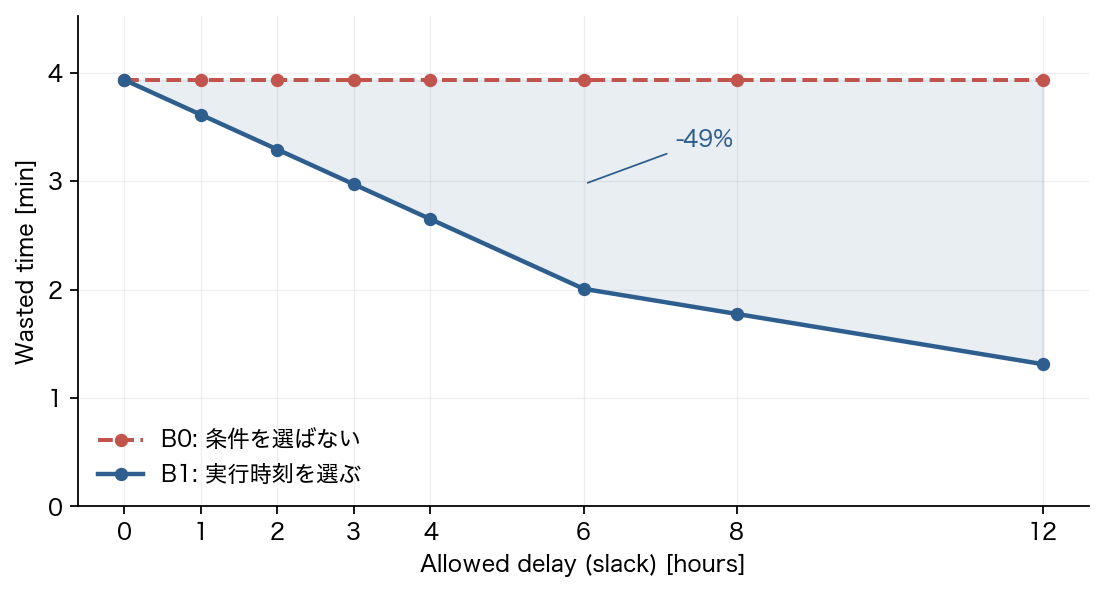
\includegraphics[width=0.85\textwidth]{images/figure6_strategy.png}
\caption{許容遅延に対する損失時間。
slack が大きいほど選択できる時間帯が増え，損失時間が減少する。}
\label{fig:strategy}
\end{figure}

許容遅延が 6 時間のとき，実行時刻の選択により
損失時間は $3.94$ 分から $2.11$ 分へ\textbf{$46\%$ 削減}され，
完了確率は $0.841$ から $0.883$ へ改善した．

\subsection{効果の頑健性}
\label{sec:holdout}

前節の評価は，条件の選択と効果の測定に
同一のデータを用いている．
このため観測期間内の偶然を効果として計上している可能性がある．

これを検証するため，観測期間を前半 4 日と後半 3 日に分割し，
\textbf{前半のデータのみで条件を選択し，後半のデータで評価する}
手続きを行った．結果を表~\ref{tab:holdout} に示す．

\begin{table}[htbp]
\centering
\caption{期間分割による検証（$d = 60$ 分，slack $=$ 6 時間）}
\label{tab:holdout}
\small
\begin{tabular}{@{}lrrr@{}}
\toprule
戦略 & 選択期間での値 & \textbf{評価期間での値} & 評価期間での削減 \\
\midrule
B0 & 8.39 分 & 1.34 分 & --- \\
B1 & 3.38 分 & \textbf{0.94 分} & $\mathbf{-30\%}$ \\
\bottomrule
\end{tabular}
\end{table}

評価期間においても B1 は B0 に対して $30\%$ の削減を示した．
\textbf{効果が観測期間内の偶然のみによるものではない}ことが確認された．

なお両期間で絶対値が大きく異なるのは，
中断の発生が期間によって偏るためである．
この変動の大きさ自体が，
単一週の観測に基づく推定の不確実性を示している．

\subsection{実行場所の選択とその限界}
\label{sec:b2_limit}

リージョンおよびインスタンスタイプまで選択範囲を広げた場合
（戦略 B2，B3）の結果を表~\ref{tab:b2_result} に示す．

\begin{table}[htbp]
\centering
\caption{選択範囲を広げた場合の損失時間（$d = 60$ 分，slack $=$ 6 時間）}
\label{tab:b2_result}
\small
\begin{tabular}{@{}llrr@{}}
\toprule
戦略 & 選択範囲 & 損失時間 & 削減率 \\
\midrule
B0 & なし & 3.94 分 & --- \\
B1 & 時刻 & 2.11 分 & $-46\%$ \\
B2 & 場所（リージョン・タイプ） & 0.10 分 & $-97\%$ \\
B3 & 時刻 $+$ 場所 & 0.08 分 & $-98\%$ \\
\bottomrule
\end{tabular}
\end{table}

B2 および B3 は B1 を大きく上回る削減を示している．
しかし\textbf{この値はそのまま受け取るべきではない}．

B2 と B3 が選択するのは Tokyo の Night 期間であるが，
この条件では観測期間中に\textbf{中断が一件も発生していない}
（$n = 42$，中断 0 件）．
このため完了確率の推定値は $1.00$ となり，
損失時間はほぼ $0$ に評価される．

問題は，48 条件のうち\textbf{15 条件（$31\%$）で
中断が一件も観測されていない}ことである．
中断 117 件が 48 条件に分散するため，
$n \approx 40$ の標本では偶然 0 件となる条件が多数生じる．
したがって完了確率 $1.00$ は
「中断しない」ことではなく「観測されなかった」ことを意味する．

\paragraph{本論文の立場．}
以上より，本論文では\textbf{B1（実行時刻の選択）を主たる結果とする}．
B1 は同一リージョン内の時間帯比較であり，
比較するすべての時間帯で中断が実際に観測されている
（表~\ref{tab:period_var}）．

一方 B2 および B3 については，
さらなる削減の余地を示唆するにとどめ，
確定的な結論は述べない．
これらの確認には標本数の増加が必要であり，
第~\ref{chap:exp} 章の実証実験の対象とする．

\section{考察}

\subsection{なぜ実行条件の選択が有効か}

\S\ref{sec:hazard} で観測されたハザード率の挙動が，
本章の結果を説明する．

中断ハザード率が経過時間によらずほぼ一定であることは，
中断リスクが\textbf{稼働時間の長さではなく
実行条件によって決まる}ことを意味する．
したがって中断されにくい条件を選べば，
その低いリスクが実行期間を通じて維持される．

\subsection{実務上の含意}

本章のモデルは，実務者に対して次の手続きを与える．

\begin{enumerate}
  \item 対象環境において $\Fcomp(d)$ と $\bar u$ を測定する
        （第~\ref{chap:measure} 章の枠組みによる）．
  \item ジョブの許容遅延と所要時間から slack を求める．
  \item 式~\eqref{eq:opt} を解き，実行条件を選択する．
\end{enumerate}

この手続きはプロバイダ固有の指標を必要とせず，
自身の観測データのみに基づく．
また最もリスクの高い時間帯はリージョンによって異なるため，
単一の普遍的な規則を適用するのではなく，
対象環境での測定に基づいて決定すべきである．

\section{本章のまとめ}

\begin{enumerate}
  \item 定期分割は，チェックポイントコストが $60$ 秒を超えると
        利得が失われ，$180$ 秒では無対策の約 $10$ 倍の損失時間が生じる．
        またワークロードの改変を要するため，本研究では採用しない．
  \item 実行条件選択のモデルを構築した．
        入力はすべて実測値であり，
        プロバイダ固有の指標を必要としない．
  \item 実行時刻の選択により損失時間は $46\%$ 削減され
        （slack $=$ 6 時間），完了確率は $0.841$ から $0.883$ へ改善する．
  \item 期間分割による検証により，
        評価期間においても $30\%$ の削減が確認された．
  \item 実行場所まで選択範囲を広げるとさらなる削減が示唆されるが，
        中断が観測されなかった条件に依存するため，
        確定的な結論は得られない．
\end{enumerate}

% =============================================================================
\chapter{実証実験}
\label{chap:exp}

\section{本章のねらい}

第~\ref{chap:model} 章の評価は，
第~\ref{chap:measure} 章で取得した観測データに基づく
シミュレーションである．
実際のワークロードを実行して得た結果ではない．

本章では，構築したモデルを実環境で検証する
実証実験の方法を示す．

\section{検証すべき事項}

\begin{table}[htbp]
\centering
\caption{実証実験で検証すべき事項}
\label{tab:objectives}
\small
\begin{tabularx}{\textwidth}{@{}clX@{}}
\toprule
優先 & 検証事項 & 理由 \\
\midrule
1 & \textbf{実行時刻選択の効果}
  & 本論文の主たる主張。
    予測値（損失時間 $-46\%$，完了確率 $+4.2$ ポイント）が
    実環境で再現されるか \\
\addlinespace
2 & モデルの予測精度
  & 式~\eqref{eq:waste} による予測値と実測値の乖離。
    モデルが現実を説明できているかを直接示す \\
\addlinespace
3 & 実行場所の選択
  & \S\ref{sec:b2_limit} で確定できなかった効果 \\
\addlinespace
4 & 中断の独立性
  & 期待試行回数 $1/p$ の前提 \\
\bottomrule
\end{tabularx}
\end{table}

\section{実験方法}

\subsection{比較の方法}

対照群と処理群を並行して実行する．

\begin{table}[htbp]
\centering
\caption{実証実験の設計}
\label{tab:exp_design}
\small
\begin{tabularx}{\textwidth}{@{}lX@{}}
\toprule
項目 & 内容 \\
\midrule
対照群（B0） & 到着時刻にそのまま実行する \\
\addlinespace
処理群（B1） & \S\ref{sec:procedure} の手続きに従い，
               許容遅延 6 時間以内で決定された時刻に実行する \\
\addlinespace
リージョン & N.~Virginia（固定） \\
インスタンスタイプ & c6a.large（固定） \\
ジョブの所要時間 & 60 分 \\
到着時刻 & 毎時 0 分（1 日 24 回，両群で 48 件） \\
\bottomrule
\end{tabularx}
\end{table}

リージョンとインスタンスタイプを固定するのは，
\S\ref{sec:b2_limit} で述べたとおり
実行場所の選択が標本数の制約を受けるためである．
本実験ではまず\textbf{実行時刻の効果のみを分離して検証する}．

両群を同一期間に並行して実行することにより，
スポット市場の時期的変動が両群に等しく影響するようにする．
これにより，観測された差を戦略の効果として解釈できる．

\subsection{実験手順}

\begin{enumerate}
  \item \textbf{テーブルの構築．}
        第~\ref{chap:measure} 章の観測データから，
        実行条件ごとの $p$，$\tilde p$，$\bar u$ を算出し保持する．
  \item \textbf{到着の発生．}
        毎時 0 分にジョブの到着を発生させる．
  \item \textbf{条件の決定．}
        対照群は遅延 $0$，処理群は
        \S\ref{sec:procedure} の手続きにより遅延を決定する．
        このとき\textbf{モデルによる予測値を記録する}．
  \item \textbf{実行．}
        決定された時刻にスポットインスタンスを起動し，
        $60$ 分間の稼働を試みる．
        待機が必要な場合は起動予約のみを登録し，
        計算資源を占有しない．
  \item \textbf{記録．}
        起動成否，中断の有無，稼働時間，
        再実行回数を記録する．
\end{enumerate}

\subsection{測定項目}

\begin{itemize}
  \item 完了率：期限 $60$ 分までに中断されなかった割合
  \item 中断回数および再実行回数
  \item 損失時間：中断された試行で費やされた時間の合計
  \item 完了までの実時間（待機時間を含む）
  \item モデルによる予測値（決定時に記録）
\end{itemize}

\subsection{必要標本数}

必要な標本数は，検証する指標によって異なる．

\paragraph{完了率を主指標とする場合．}
完了確率の差（$4.2$ ポイント）を
有意水準 $5\%$，検出力 $80\%$ で検出するには，
両群合計で約 $2{,}160$ 件を要する\footnote{%
二標本比率の検定における標本サイズの近似式
$n \approx 16\,\bar p(1-\bar p)/\delta^{2}$（片群あたり）による。
$\bar p = 0.862$，$\delta = 0.042$ として片群約 $1{,}079$ 件。}．
1 日 48 件を実行する場合，\textbf{約 45 日}を要する．

\paragraph{損失時間を主指標とする場合．}
損失時間は $46\%$ 減少すると予測され，
完了率より大きな相対差を持つ．
ただし損失時間は中断が発生した場合にのみ正の値をとるため，
必要標本数は中断の発生件数に依存する．

\paragraph{実験期間の設定．}
以上より\textbf{最低 6 週間（両群計約 $2{,}000$ 件）}を基本とし，
中間時点で効果量を確認したうえで延長の要否を判断する．
曜日による変動を考慮し，期間は 7 日の整数倍とする．

所要コストは，c6a.large の観測スポット価格
（$0.0295$ USD/h）に基づくと約 \textbf{\$64} である．

\section{実装方針}

第~\ref{chap:measure} 章で構築した測定フレームワークを流用する．
必要な変更を表~\ref{tab:impl} に示す．

\begin{table}[htbp]
\centering
\caption{既存実装からの変更点}
\label{tab:impl}
\small
\begin{tabularx}{\textwidth}{@{}lX@{}}
\toprule
要素 & 変更内容 \\
\midrule
決定処理 & \S\ref{sec:procedure} の手続きを実装し，
           事前に構築したテーブルを参照して起動時刻を決定する \\
\addlinespace
遅延実行 & 決定された時刻に起動するための予約機構を追加する。
           待機中に計算資源を占有しないよう，
           イベントスケジューラへの登録のみを行う \\
\addlinespace
中断検知 & 既存の実装をそのまま流用する \\
\addlinespace
記録項目 & 群の識別子，到着時刻，実際の遅延時間，
           および決定時の予測値を追加する \\
\bottomrule
\end{tabularx}
\end{table}

遅延実行の機構が唯一の新規実装となる．
本実験に先立ち，小規模な動作確認を行う．

\section{想定される結果}

\begin{table}[htbp]
\centering
\caption{実験結果に応じた結論}
\label{tab:outcomes}
\small
\begin{tabularx}{\textwidth}{@{}lX@{}}
\toprule
実測結果 & 導かれる結論 \\
\midrule
予測と整合する
  & 実行条件の選択が有効であり，
    式~\eqref{eq:waste} が実環境を説明できることが示される \\
\addlinespace
効果はあるが予測より小さい
  & 効果の存在は確認されるが，モデルの前提
    （とりわけ試行の独立性）に修正が必要となる \\
\addlinespace
効果が認められない
  & 観測期間と実験期間の間でスポット市場が変化したか，
    単一週の観測に基づく推定が一般化できないことを示す。
    \textbf{観測結果の有効期間}という新たな問いが生じる \\
\bottomrule
\end{tabularx}
\end{table}

\section{想定されるリスク}

\begin{table}[htbp]
\centering
\caption{想定されるリスクと対策}
\label{tab:risks}
\small
\begin{tabularx}{\textwidth}{@{}XXX@{}}
\toprule
リスク & 影響 & 対策 \\
\midrule
中断が十分に集まらない
  & 検出力の不足
  & 期間の延長により標本数を確保する \\
\addlinespace
観測期間と実験期間の市場変化
  & 予測が外れる
  & 実験期間中に $\Fcomp$ を再測定し比較する \\
\addlinespace
独立性が成立しない
  & $p$ が過大評価となる
  & 中断直後の再試行の成否を記録する \\
\addlinespace
遅延実行機構の不具合
  & 実験全体が無効となる
  & 事前に小規模な動作確認を行う \\
\bottomrule
\end{tabularx}
\end{table}

% =============================================================================
\chapter{結論}
\label{chap:conclusion}

\section{本論文のまとめ}

本論文は，スポットインスタンス上の短時間ワークロードにおいて，
\textbf{中断によって失われる時間を最小化する実行条件を
どう決定するか}という問いに取り組んだ．

既存研究では SPS のようなプロバイダ固有の指標に基づく
実行先の選択が検討されてきた．
しかし SPS は起動のしやすさを示す指標であり，
起動後の継続性を示すものではない．
第~\ref{chap:prelim} 章では，この課題認識を
予備実験により確認した．

第~\ref{chap:measure} 章では，実測値のみから算出される
信頼性指標として期限条件付き完了可能性 $\Fcomp(d)$ を定義し，
AWS の 4 リージョン・3 インスタンスタイプを対象として
1 週間の実測（$\Nreq = 2{,}016$）を行った．
$\Fcomp(60)$ は実行条件によって $0.69$--$1.00$ の範囲で変動し，
最大の差は N.~Virginia の c6a.large における
Night 期間と Morning 期間の間の $0.29$ であった．
また中断ハザード率は経過時間によらずほぼ一定であった．

第~\ref{chap:model} 章では，これらの観測に基づき
実行条件選択モデルを構築した．

中断時の損失を抑える手法として定期分割も検討したが，
チェックポイントコストが $60$ 秒を超えると利得が失われ，
$180$ 秒では無対策の約 $10$ 倍の損失時間が生じる．
またワークロードの改変を要するため，本研究では採用しない．

採用した実行条件選択モデルは，
ワークロードの改変を必要とせず，
入力はすべて実測値である．
実行時刻の選択により損失時間は $46\%$ 削減され，
完了確率は $0.841$ から $0.883$ へ改善した．
期間分割による検証により，
評価期間においても $30\%$ の削減が確認された．

第~\ref{chap:exp} 章では，構築したモデルを
実環境で検証する実証実験の方法を示した．

\section{本研究の意義}

\begin{enumerate}
  \item スポットインスタンスの信頼性を，
        プロバイダ固有の不透明な指標ではなく，
        直接観測された起動・中断記録のみから算出される
        \textbf{解釈可能な指標}として定式化した．
  \item 従来は観測・記述の対象として扱われてきた
        中断挙動の変動を，
        \textbf{実行条件を選択するための入力}として
        利用する枠組みを与えた．
  \item 広く行われている定期チェックポイント取得が，
        保存コストの大きいワークロードでは
        \textbf{かえって損失時間を増大させる}ことを
        定量的に示した．
  \item 提案手法は\textbf{ワークロード自体の改変を必要としない}．
        実務上の導入障壁が低い．
\end{enumerate}

\section{今後の課題}

\begin{itemize}
  \item 第~\ref{chap:exp} 章で示した実証実験の実施
  \item 観測期間の延長による長期的傾向の把握，
        および観測結果の有効期間の検討
  \item 実行場所の選択（B2・B3）の効果の確定
  \item 中断の独立性の検証と，成立しない場合のモデルの修正
  \item 定期分割との併用効果の検討
\end{itemize}

% =============================================================================
\chapter*{謝辞}
\addcontentsline{toc}{chapter}{謝辞}

本研究を進めるにあたり，終始丁寧なご指導を賜りました
指導教員の先生方に深く感謝いたします．
また，日頃より有益な議論をいただいた研究室の皆様に御礼申し上げます．

% =============================================================================
\begin{thebibliography}{99}
\addcontentsline{toc}{chapter}{参考文献}

\bibitem{AWSSpot}
Amazon Web Services:
Amazon EC2 Spot Instances.
\url{https://aws.amazon.com/ec2/spot/}
(Accessed: May 2026)

\bibitem{Lin2022Survey}
Lin, L., Pan, L., Liu, S.:
Methods for improving the availability of spot instances: A survey.
Computers in Industry, 141, 103718 (2022).

\bibitem{Ramesh2025}
Ramesh, D.G.A., Lennon, R.G.:
Evaluating the Impact of Reserved Instances vs. Spot Instances in DevOps Cloud Workflows.
In: 2025 35th Irish Signals and Systems Conference (ISSC). IEEE (2025).

\bibitem{Garg2025}
Garg, D., Kaata, S.K., Bhumireddy, D.R., Bolla, B.K.:
Reducing Cloud Cost Through Optimized Bidding for AWS Spot Instances.
In: 2025 3rd International Conference on Advances in Computation,
Communication and Information Technology (ICAICCIT). IEEE (2025).

\bibitem{Katayama2022}
Katayama, D., Kasai, K., Koita, T.:
Migration Destination Selection Algorithm for Spot Instances using SPS.
In: 2022 IEEE International Conference on Big Data (Big Data),
pp. 6690--6692. IEEE, Osaka (2022).

\bibitem{Kim2024SpotInterruption}
Kim, K., Lee, K.:
Making Cloud Spot Instance Interruption Events Visible.
In: Proceedings of the ACM Web Conference 2024 (WWW '24),
pp. 2998--3009. ACM, New York (2024).

\bibitem{AWSSPS}
Amazon Web Services:
Spot Placement Score. Amazon EC2 User Guide.
\url{https://docs.aws.amazon.com/AWSEC2/latest/UserGuide/spot-placement-score.html}
(Accessed: May 2026)

\bibitem{Lee2022SpotLake}
Lee, S., Hwang, J., Lee, K.:
SpotLake: Diverse Spot Instance Dataset Archive Service.
In: 2022 IEEE International Symposium on Workload Characterization (IISWC),
pp. 242--255. IEEE (2022).

\bibitem{Pham2018}
Pham, T.-P., Ristov, S., Fahringer, T.:
Performance and Behavior Characterization of Amazon EC2 Spot Instances.
In: 2018 IEEE 11th International Conference on Cloud Computing (CLOUD).
IEEE (2018).

\bibitem{AWSInstanceTypes}
Amazon Web Services:
Amazon EC2 Instance Types. Amazon EC2 User Guide.
\url{https://docs.aws.amazon.com/AWSEC2/latest/UserGuide/instance-types.html}
(Accessed: May 2026)

\end{thebibliography}

\end{document}
